\documentclass[11pt]{article}
\usepackage[notes]{la}
\lamodule{6}{1}{Inner Product, Length, and Orthogonality}
\laxdoc{1.4}
\laxdoc{2.1}
\laxdoc{4.1}
\laxdoc{4.2}

\begin{document}

\section{Inner Product, Length, and Orthogonality}

\begin{guide}
Up to now a vector has been a list of numbers that we add and scale. Nothing so far lets us say how long a vector is, how far one vector is from another, or whether two vectors meet at a right angle. All three questions are answered by one operation that turns two vectors into a single number: the dot product. This section defines it, shows that it obeys four simple rules, and then uses those rules, and nothing else, to build length, distance, perpendicularity and the angle between two vectors. At the end we ask which vectors are perpendicular to a whole subspace, and we find that the answer is a null space we already know how to compute.
\end{guide}

\textbf{By the end of this section you should be able to:}
\begin{itemize}
  \item compute the dot product of two vectors in $\R^n$ and use its four rules to expand and simplify expressions;
  \item find the length of a vector, a unit vector in a given direction, and the distance between two vectors;
  \item decide whether two vectors are orthogonal, and use the Pythagorean theorem in $\R^n$;
  \item state and use the Cauchy--Schwarz and triangle inequalities, and compute the angle between two vectors;
  \item find the orthogonal complement of a subspace, in particular of the span of given vectors, of $\Row A$ and of $\Col A$.
\end{itemize}

% ---------------------------------------------------------------------
\subsection*{The inner product}

Two vectors $\bv{u}$ and $\bv{v}$ in $\R^n$ are $n\times1$ matrices. The transpose $\bv{u}\T$ is a $1\times n$ matrix (Definition~\ref{2.1-def:transpose}), so the product $\bv{u}\T\bv{v}$ is a $1\times1$ matrix, which we read as an ordinary number.

\begin{exmp}{A dot product as a matrix product}{dot1}
Let $\bv{u}=(3,-1,2)$ and $\bv{v}=(4,5,-2)$. Then
\[
\bv{u}\T\bv{v}=\begin{bmatrix}3&-1&2\end{bmatrix}\begin{bmatrix}4\\5\\-2\end{bmatrix}=(3)(4)+(-1)(5)+(2)(-2)=12-5-4=3.
\]
Reversing the order gives the same number: $\bv{v}\T\bv{u}=(4)(3)+(5)(-1)+(-2)(2)=12-5-4=3$. The number is a sum of products of corresponding entries.
\end{exmp}

\begin{defn}{Inner product (dot product)}{dot}
For $\bv{u}=(u_1,\dots,u_n)$ and $\bv{v}=(v_1,\dots,v_n)$ in $\R^n$, the \emph{inner product} (or \emph{dot product}) is the number
\[
\bv{u}\cdot\bv{v}=\bv{u}\T\bv{v}=u_1v_1+u_2v_2+\cdots+u_nv_n .
\]
\end{defn}

It is also written $\inner{\bv{u}}{\bv{v}}$. The result is a \emph{scalar}, not a vector, and the two vectors must have the same number of entries. Dot products appear whenever we add up ``quantity times rate'':

\begin{exmp}{A dot product as a total cost}{cost}
A kitchen buys $10$ kg of rice, $4$ kg of beans and $6$ kg of lentils, at the prices $2$, $3$ and $5$ dollars per kg. With $\bv{p}=(2,3,5)$ and $\bv{q}=(10,4,6)$, the total cost is $\bv{p}\cdot\bv{q}=(2)(10)+(3)(4)+(5)(6)=20+12+30=62$ dollars.
\end{exmp}

The dot product has four properties, and everything in this section follows from them.

\begin{thm}{Properties of the inner product}{dotprops}
Let $\bv{u},\bv{v},\bv{w}$ be vectors in $\R^n$ and let $c$ be a scalar. Then
\begin{enumerate}[label=(\alph*),itemsep=1pt]
  \item $\bv{u}\cdot\bv{v}=\bv{v}\cdot\bv{u}$;
  \item $(\bv{u}+\bv{v})\cdot\bv{w}=\bv{u}\cdot\bv{w}+\bv{v}\cdot\bv{w}$;
  \item $(c\bv{u})\cdot\bv{v}=c(\bv{u}\cdot\bv{v})=\bv{u}\cdot(c\bv{v})$;
  \item $\bv{u}\cdot\bv{u}\ge0$, and $\bv{u}\cdot\bv{u}=0$ if and only if $\bv{u}=\bv{0}$.
\end{enumerate}
\end{thm}

\begin{proof}
(a)~$\bv{u}\cdot\bv{v}=\sum u_iv_i=\sum v_iu_i=\bv{v}\cdot\bv{u}$, because multiplication of numbers is commutative.

(b)~$(\bv{u}+\bv{v})\cdot\bv{w}=\sum(u_i+v_i)w_i=\sum u_iw_i+\sum v_iw_i=\bv{u}\cdot\bv{w}+\bv{v}\cdot\bv{w}$.

(c)~$(c\bv{u})\cdot\bv{v}=\sum(cu_i)v_i=c\sum u_iv_i=c(\bv{u}\cdot\bv{v})$, and in the same way $\bv{u}\cdot(c\bv{v})=\sum u_i(cv_i)=c(\bv{u}\cdot\bv{v})$.

(d)~$\bv{u}\cdot\bv{u}=u_1^2+\cdots+u_n^2$ is a sum of squares of real numbers, so it is at least $0$. It equals $0$ only if every square is $0$, that is, only if every $u_i=0$.
\end{proof}

Rules (b) and (c) can be combined: the dot product of two sums of multiples is the sum of all the products of multiples, exactly as in multiplying out brackets. By (a) the order does not matter.

\begin{exmp}{Multiplying out}{expand}
Suppose $\bv{u}\cdot\bv{u}=5$, $\bv{v}\cdot\bv{v}=2$ and $\bv{u}\cdot\bv{v}=-1$. Then
\[
(2\bv{u}-3\bv{v})\cdot(\bv{u}+4\bv{v})=2\,\bv{u}\cdot\bv{u}+8\,\bv{u}\cdot\bv{v}-3\,\bv{v}\cdot\bv{u}-12\,\bv{v}\cdot\bv{v}=2(5)+8(-1)-3(-1)-12(2)=10-8+3-24=-19.
\]
We never needed the entries of $\bv{u}$ and $\bv{v}$; the rules were enough.
\end{exmp}

\begin{think}{Reading the definition}{dotstruct}
(a)~What is $\bv{u}\cdot\bv{e}_j$ for a vector $\bv{u}$ in $\R^n$? (b)~Why can we not take the dot product of a vector in $\R^2$ with a vector in $\R^3$? (c)~Why does the expression $\bv{u}\cdot\bv{v}\cdot\bv{w}$ make no sense?
\end{think}

\begin{think}{Moving a matrix across a dot product}{movemat}
(a)~Use Theorem~\ref{2.1-thm:transprops}(d) to show that $(A\bv{x})\cdot\bv{y}=\bv{x}\cdot(A\T\bv{y})$ for every $m\times n$ matrix $A$, $\bv{x}$ in $\R^n$ and $\bv{y}$ in $\R^m$. (b)~Check it for $A=\begin{bmatrix}1&2\\0&3\end{bmatrix}$, $\bv{x}=(1,1)$ and $\bv{y}=(2,-1)$.
\end{think}

\begin{kc}{Dot products}{kcdot}
Compute (a)~$(1,-2,3)\cdot(4,0,-1)$; (b)~$(2,5)\cdot(-5,2)$; (c)~$(2,-1,0,3)\cdot(1,1,1,1)$.
\end{kc}

% ---------------------------------------------------------------------
\subsection*{Length and distance}

In $\R^2$ the vector $\bv{v}=(a,b)$ is the arrow from the origin to the point $(a,b)$. By the Pythagorean theorem the arrow has length $\sqrt{a^2+b^2}$, which is $\sqrt{\bv{v}\cdot\bv{v}}$. The same formula defines length in every $\R^n$, and it makes sense because $\bv{v}\cdot\bv{v}\ge0$ by Theorem~\ref{thm:dotprops}(d).

\begin{defn}{Length, unit vector and distance}{len}
The \emph{length} (or \emph{norm}) of $\bv{v}$ in $\R^n$ is the nonnegative number
\[
\lVert\bv{v}\rVert=\sqrt{\bv{v}\cdot\bv{v}}=\sqrt{v_1^2+v_2^2+\cdots+v_n^2},\qquad\text{so that}\qquad\lVert\bv{v}\rVert^2=\bv{v}\cdot\bv{v}.
\]
A \emph{unit vector} is a vector of length $1$. The \emph{distance} between $\bv{u}$ and $\bv{v}$ is $\operatorname{dist}(\bv{u},\bv{v})=\lVert\bv{u}-\bv{v}\rVert$.
\end{defn}

\begin{center}
\begin{tikzpicture}[>=stealth,scale=0.7]
  \draw[gray!50,->] (-0.5,0)--(5,0);
  \draw[gray!50,->] (0,-0.5)--(0,5);
  \draw[->,thick,blue] (0,0)--(3,4) node[above right] {v = (3,4)};
  \draw[dashed] (3,0)--(3,4);
  \draw (2.7,0)--(2.7,0.3)--(3,0.3);
  \node at (1.5,-0.4) {3};
  \node at (3.4,2) {4};
  \node at (1.0,2.5) {length 5};
  \draw[->,thick,red] (8,1)--(10,4.5);
  \node at (7.7,0.7) {u};
  \node at (10.3,4.8) {v};
  \draw[dashed] (8,1)--(10,4.5) node[midway,right] {dist};
\end{tikzpicture}
\end{center}

\noindent\textbf{Figure 1.} Left: the vector $(3,4)$ is the hypotenuse of a right triangle with legs $3$ and $4$, so its length is $\sqrt{9+16}=5$. Right: the distance between the points $\bv{u}$ and $\bv{v}$ is the length of the segment joining them, which is the length of $\bv{u}-\bv{v}$.

\begin{thm}{Scaling a vector}{scale}
For every scalar $c$ and every vector $\bv{v}$, $\lVert c\bv{v}\rVert=|c|\,\lVert\bv{v}\rVert$. In particular, if $\bv{v}\neq\bv{0}$ then $\bv{v}/\lVert\bv{v}\rVert$ is a unit vector.
\end{thm}

\begin{proof}
By Theorem~\ref{thm:dotprops}(c), $\lVert c\bv{v}\rVert^2=(c\bv{v})\cdot(c\bv{v})=c^2(\bv{v}\cdot\bv{v})=c^2\lVert\bv{v}\rVert^2$, and the square root of $c^2$ is $|c|$. If $\bv{v}\neq\bv{0}$ then $\lVert\bv{v}\rVert>0$ by Theorem~\ref{thm:dotprops}(d); taking $c=1/\lVert\bv{v}\rVert$ gives $\lVert\bv{v}/\lVert\bv{v}\rVert\rVert=\lVert\bv{v}\rVert/\lVert\bv{v}\rVert=1$.
\end{proof}

\begin{proc}{A unit vector in the direction of $\bv{v}$}{unit}
\begin{enumerate}[nosep]
  \item Compute $\bv{v}\cdot\bv{v}$, the sum of the squares of the entries.
  \item Take the square root to get $\lVert\bv{v}\rVert$ (it must be positive, since $\bv{v}\neq\bv{0}$).
  \item Divide: $\bv{u}=\bv{v}/\lVert\bv{v}\rVert$. This is called \emph{normalizing} $\bv{v}$.
  \item Check: $\bv{u}\cdot\bv{u}=1$.
\end{enumerate}
\end{proc}

\begin{exmp}{Length and a unit vector}{len1}
For $\bv{v}=(2,3,-6)$ we have $\bv{v}\cdot\bv{v}=4+9+36=49$, so $\lVert\bv{v}\rVert=7$ and the unit vector in the direction of $\bv{v}$ is $\bv{u}=\tfrac17(2,3,-6)$. Check: $\bv{u}\cdot\bv{u}=\tfrac{1}{49}(4+9+36)=1$. \ $\checkmark$
\end{exmp}

\begin{exmp}{Length in $\R^4$ and scaling}{len4}
Let $\bv{w}=(2,4,-1,2)$. Then $\lVert\bv{w}\rVert^2=4+16+1+4=25$, so $\lVert\bv{w}\rVert=5$. By Theorem~\ref{thm:scale}, $\lVert-3\bv{w}\rVert=3\cdot5=15$, and $\tfrac15(2,4,-1,2)$ is a unit vector. Length is defined in the same way in every $\R^n$, even though we cannot draw $\R^4$.
\end{exmp}

\begin{exmp}{Distance}{dist1}
The distance between $\bv{u}=(7,1,-2)$ and $\bv{v}=(3,-3,0)$: the difference is $\bv{u}-\bv{v}=(4,4,-2)$ and $\lVert\bv{u}-\bv{v}\rVert^2=16+16+4=36$, so the distance is $6$. In the plane, the points $(1,4)$ and $(-2,0)$ differ by $(3,4)$, so their distance is $\sqrt{9+16}=5$.
\end{exmp}

\begin{exmp}{Lengths from dot products alone}{normdot}
Suppose $\lVert\bv{u}\rVert=3$, $\lVert\bv{v}\rVert=2$ and $\bv{u}\cdot\bv{v}=-1$. Multiplying out as in Example~\ref{ex:expand},
\begin{align*}
\lVert\bv{u}+\bv{v}\rVert^2&=\lVert\bv{u}\rVert^2+2\,\bv{u}\cdot\bv{v}+\lVert\bv{v}\rVert^2=9+2(-1)+4=11,\\
\lVert\bv{u}-\bv{v}\rVert^2&=\lVert\bv{u}\rVert^2-2\,\bv{u}\cdot\bv{v}+\lVert\bv{v}\rVert^2=9-2(-1)+4=15,\\
\lVert2\bv{u}-\bv{v}\rVert^2&=4\lVert\bv{u}\rVert^2-4\,\bv{u}\cdot\bv{v}+\lVert\bv{v}\rVert^2=4(9)-4(-1)+4=44.
\end{align*}
\end{exmp}

\begin{think}{Scaling and signs}{unitthink}
(a)~What is $\lVert-\bv{v}\rVert$? (b)~If $\bv{v}\neq\bv{0}$, why is $-\bv{v}/\lVert\bv{v}\rVert$ also a unit vector, and in which direction does it point? (c)~Is there a nonzero vector of length $0$?
\end{think}

\begin{kc}{Length, unit vectors and distance}{kclen}
(a)~Find $\lVert(6,-2,3)\rVert$. (b)~Find a unit vector in the direction of $(6,-2,3)$. (c)~Find the distance between $(1,1,1,1)$ and $(3,-1,3,-1)$.
\end{kc}

% ---------------------------------------------------------------------
\subsection*{Orthogonal vectors}

When is the angle between $\bv{u}$ and $\bv{v}$ a right angle? Multiply out the squared length of $\bv{u}+\bv{v}$ using Theorem~\ref{thm:dotprops}:
\begin{equation}\label{eq:sumsq}
\lVert\bv{u}+\bv{v}\rVert^2=(\bv{u}+\bv{v})\cdot(\bv{u}+\bv{v})=\bv{u}\cdot\bv{u}+2\,\bv{u}\cdot\bv{v}+\bv{v}\cdot\bv{v}=\lVert\bv{u}\rVert^2+2\,\bv{u}\cdot\bv{v}+\lVert\bv{v}\rVert^2,
\end{equation}
and in the same way $\lVert\bv{u}-\bv{v}\rVert^2=\lVert\bv{u}\rVert^2-2\,\bv{u}\cdot\bv{v}+\lVert\bv{v}\rVert^2$. The lines through the origin and $\bv{u}$, and through the origin and $\bv{v}$, are perpendicular exactly when $\bv{u}$ is equally far from $\bv{v}$ and from $-\bv{v}$, that is, when $\lVert\bv{u}-\bv{v}\rVert^2=\lVert\bv{u}+\bv{v}\rVert^2$. By the two formulas this happens exactly when $-2\,\bv{u}\cdot\bv{v}=2\,\bv{u}\cdot\bv{v}$, that is, when $\bv{u}\cdot\bv{v}=0$. This is the definition we use in $\R^n$.

\begin{defn}{Orthogonal vectors}{orth}
Two vectors $\bv{u}$ and $\bv{v}$ in $\R^n$ are \emph{orthogonal} (to each other) if $\bv{u}\cdot\bv{v}=0$. We write $\bv{u}\perp\bv{v}$.
\end{defn}

The zero vector is orthogonal to every vector, because $\bv{0}\cdot\bv{v}=0$.

\begin{thm}{The Pythagorean theorem}{pyth}
Two vectors $\bv{u}$ and $\bv{v}$ in $\R^n$ are orthogonal if and only if $\lVert\bv{u}+\bv{v}\rVert^2=\lVert\bv{u}\rVert^2+\lVert\bv{v}\rVert^2$.
\end{thm}

\begin{proof}
By equation~\eqref{eq:sumsq}, $\lVert\bv{u}+\bv{v}\rVert^2-\lVert\bv{u}\rVert^2-\lVert\bv{v}\rVert^2=2\,\bv{u}\cdot\bv{v}$. This difference is $0$ if and only if $\bv{u}\cdot\bv{v}=0$.
\end{proof}

\begin{exmp}{Testing pairs}{orthtest}
$(1,2,-1)\cdot(3,-1,1)=3-2-1=0$, so these vectors are orthogonal. $(4,1,-2)\cdot(1,2,2)=4+2-4=2\neq0$, so these are not. A single nonzero dot product is enough to show that two vectors are not orthogonal.
\end{exmp}

\begin{exmp}{Finding an unknown entry}{orthc}
For which number $c$ are $(c,3,-2)$ and $(5,c,2)$ orthogonal? The dot product is $5c+3c-4=8c-4$, which is $0$ exactly when $c=\tfrac12$. Check: $\tfrac12(5)+3(\tfrac12)+(-2)(2)=\tfrac52+\tfrac32-4=0$. \ $\checkmark$
\end{exmp}

\begin{exmp}{Rotating by a quarter turn}{rot90}
In $\R^2$, for $\bv{v}=(a,b)$ the vector $(-b,a)$ is always orthogonal to $\bv{v}$, since $a(-b)+b\,a=0$. For $\bv{v}=(3,4)$ we get $(-4,3)$: $(3)(-4)+(4)(3)=-12+12=0$, and both vectors have length $5$.
\end{exmp}

\begin{exmp}{The Pythagorean theorem in numbers}{pythnum}
Let $\bv{u}=(2,1,-2)$ and $\bv{v}=(1,2,2)$. Then $\bv{u}\cdot\bv{v}=2+2-4=0$. The sum is $\bv{u}+\bv{v}=(3,3,0)$, with $\lVert\bv{u}+\bv{v}\rVert^2=18$, and $\lVert\bv{u}\rVert^2+\lVert\bv{v}\rVert^2=9+9=18$. \ $\checkmark$ For $\bv{w}=(1,2,3)$ the vectors $\bv{u}$ and $\bv{w}$ are not orthogonal: $\bv{u}\cdot\bv{w}=2+2-6=-2$, and indeed $\lVert\bv{u}+\bv{w}\rVert^2=19$ while $\lVert\bv{u}\rVert^2+\lVert\bv{w}\rVert^2=9+14=23$; the difference $19-23=-4$ is $2\,\bv{u}\cdot\bv{w}$, as equation~\eqref{eq:sumsq} predicts.
\end{exmp}

\begin{think}{Orthogonal to itself}{orthzero}
(a)~For which vector $\bv{v}$ is $\bv{v}\cdot\bv{v}=0$? (b)~Which vector is orthogonal to itself? (c)~In $\R^2$, which vectors are orthogonal to $(1,0)$? Which are orthogonal to a given nonzero vector $(a,b)$?
\end{think}

\begin{kc}{Orthogonal or not?}{kcorth}
Decide whether each pair is orthogonal. (a)~$(1,-1,2)$ and $(3,1,-1)$. (b)~$(1,2,3,4)$ and $(4,-3,2,-1)$. (c)~$(1,1,1)$ and $(1,-2,2)$. (d)~$\bv{0}$ and $(5,-7)$.
\end{kc}

% ---------------------------------------------------------------------
\subsection*{The Cauchy--Schwarz inequality and angles}

How large can $\bv{u}\cdot\bv{v}$ be, compared with the lengths of $\bv{u}$ and $\bv{v}$? The answer is also what makes the word ``angle'' meaningful in $\R^n$.

\begin{thm}{The Cauchy--Schwarz and triangle inequalities}{cs}
For all vectors $\bv{u}$ and $\bv{v}$ in $\R^n$:
\begin{enumerate}[label=(\alph*),itemsep=1pt]
  \item $|\bv{u}\cdot\bv{v}|\le\lVert\bv{u}\rVert\,\lVert\bv{v}\rVert$;
  \item $\lVert\bv{u}+\bv{v}\rVert\le\lVert\bv{u}\rVert+\lVert\bv{v}\rVert$.
\end{enumerate}
\end{thm}

\begin{proof}
(a)~If $\bv{v}=\bv{0}$ both sides are $0$. Otherwise let $t=(\bv{u}\cdot\bv{v})/(\bv{v}\cdot\bv{v})$. By Theorem~\ref{thm:dotprops}(d) and the rules of that theorem,
\[
0\le\lVert\bv{u}-t\bv{v}\rVert^2=\bv{u}\cdot\bv{u}-2t\,\bv{u}\cdot\bv{v}+t^2\,\bv{v}\cdot\bv{v}=\lVert\bv{u}\rVert^2-\frac{(\bv{u}\cdot\bv{v})^2}{\lVert\bv{v}\rVert^2}.
\]
Hence $(\bv{u}\cdot\bv{v})^2\le\lVert\bv{u}\rVert^2\lVert\bv{v}\rVert^2$, and taking square roots gives (a).

(b)~By equation~\eqref{eq:sumsq} and part (a), $\lVert\bv{u}+\bv{v}\rVert^2=\lVert\bv{u}\rVert^2+2\,\bv{u}\cdot\bv{v}+\lVert\bv{v}\rVert^2\le\lVert\bv{u}\rVert^2+2\lVert\bv{u}\rVert\lVert\bv{v}\rVert+\lVert\bv{v}\rVert^2=\bigl(\lVert\bv{u}\rVert+\lVert\bv{v}\rVert\bigr)^2$. Taking square roots of the two nonnegative sides gives (b).
\end{proof}

Part (b) says that the straight segment is the shortest route: going from the origin to $\bv{u}+\bv{v}$ directly is never longer than going to $\bv{u}$ first and then along $\bv{v}$.

For nonzero $\bv{u}$ and $\bv{v}$ in $\R^2$, the law of cosines in the triangle with sides $\bv{u}$, $\bv{v}$ and $\bv{u}-\bv{v}$ gives $\lVert\bv{u}-\bv{v}\rVert^2=\lVert\bv{u}\rVert^2+\lVert\bv{v}\rVert^2-2\lVert\bv{u}\rVert\lVert\bv{v}\rVert\cos\theta$. Comparing with the formula for $\lVert\bv{u}-\bv{v}\rVert^2$ above shows that $\bv{u}\cdot\bv{v}=\lVert\bv{u}\rVert\lVert\bv{v}\rVert\cos\theta$. We use this as the definition of the angle in $\R^n$: for nonzero $\bv{u}$ and $\bv{v}$,
\[
\cos\theta=\frac{\bv{u}\cdot\bv{v}}{\lVert\bv{u}\rVert\,\lVert\bv{v}\rVert},\qquad 0^\circ\le\theta\le180^\circ.
\]
Theorem~\ref{thm:cs}(a) says that the fraction lies between $-1$ and $1$, so such a $\theta$ exists. The angle is $90^\circ$ exactly when $\bv{u}\cdot\bv{v}=0$.

\begin{exmp}{An angle in $\R^3$}{angle}
For $\bv{u}=(1,1,0)$ and $\bv{v}=(0,1,1)$: $\bv{u}\cdot\bv{v}=1$ and $\lVert\bv{u}\rVert=\lVert\bv{v}\rVert=\sqrt2$, so $\cos\theta=1/2$ and $\theta=60^\circ$. For $\bv{u}=(1,-2,2)$ and $\bv{v}=(2,1,-2)$: $\bv{u}\cdot\bv{v}=2-2-4=-4$ and $\lVert\bv{u}\rVert=\lVert\bv{v}\rVert=3$, so $\cos\theta=-4/9$ and $\theta\approx116.4^\circ$. A negative dot product means an obtuse angle.
\end{exmp}

\begin{exmp}{Checking the inequalities}{csnum}
Let $\bv{u}=(1,-2,2)$ and $\bv{v}=(4,3,0)$. Then $\bv{u}\cdot\bv{v}=4-6+0=-2$, $\lVert\bv{u}\rVert=3$ and $\lVert\bv{v}\rVert=5$, so $|\bv{u}\cdot\bv{v}|=2\le15$. Also $\bv{u}+\bv{v}=(5,1,2)$ has length $\sqrt{30}\approx5.48\le3+5=8$. Equality in Cauchy--Schwarz occurs when one vector is a multiple of the other: for $\bv{v}=2\bv{u}=(2,-4,4)$, $\bv{u}\cdot\bv{v}=2+8+8=18=3\cdot6=\lVert\bv{u}\rVert\lVert\bv{v}\rVert$.
\end{exmp}

\begin{think}{When is it an equality?}{csthink}
(a)~In the proof of Theorem~\ref{thm:cs}(a), what must be true of $\bv{u}-t\bv{v}$ if equality holds? (b)~So when does $|\bv{u}\cdot\bv{v}|=\lVert\bv{u}\rVert\lVert\bv{v}\rVert$ hold, for $\bv{v}\neq\bv{0}$?
\end{think}

\begin{kc}{Angles and the inequality}{kcangle}
(a)~Find the angle between $(1,0,1)$ and $(1,1,0)$. (b)~Find the angle between $(1,-1)$ and $(-2,2)$. (c)~Can there be vectors $\bv{u},\bv{v}$ in $\R^3$ with $\bv{u}\cdot\bv{v}=10$, $\lVert\bv{u}\rVert=2$ and $\lVert\bv{v}\rVert=4$?
\end{kc}

% ---------------------------------------------------------------------
\subsection*{Orthogonal complements}

\begin{defn}{Orthogonal complement}{perp}
Let $W$ be a subspace of $\R^n$. A vector $\bv{z}$ is \emph{orthogonal to $W$} if $\bv{z}\cdot\bv{w}=0$ for every $\bv{w}$ in $W$. The set of all vectors orthogonal to $W$ is the \emph{orthogonal complement} of $W$, written $W^{\perp}$ (read ``$W$ perp'').
\end{defn}

\begin{exmp}{Two easy complements}{planeperp}
Let $W=\Span\{(1,0,0),(0,1,0)\}$, the $x_1x_2$-plane in $\R^3$. A vector $\bv{z}$ is orthogonal to both $(1,0,0)$ and $(0,1,0)$ exactly when $z_1=0$ and $z_2=0$, and then $\bv{z}\cdot\bv{w}=0$ for every $\bv{w}$ in $W$. So $W^{\perp}=\Span\{(0,0,1)\}$, the $x_3$-axis. In $\R^2$ let $W=\Span\{(2,1)\}$. Then $(z_1,z_2)\perp(2,1)$ means $2z_1+z_2=0$, so $\bv{z}=z_1(1,-2)$ and $W^{\perp}=\Span\{(1,-2)\}$.
\end{exmp}

\begin{center}
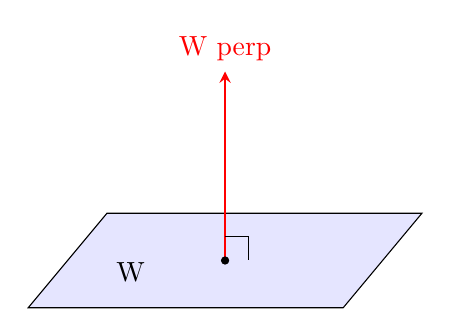
\begin{tikzpicture}[>=stealth]
  \draw[fill=blue!10] (0,0)--(4,0)--(5,1.2)--(1,1.2)--cycle;
  \node at (1.3,0.45) {W};
  \draw[->,thick,red] (2.5,0.6)--(2.5,3) node[above] {W perp};
  \draw (2.5,0.9)--(2.8,0.9)--(2.8,0.6);
  \fill (2.5,0.6) circle (1.5pt);
\end{tikzpicture}
\end{center}

\noindent\textbf{Figure 2.} A plane $W$ through the origin in $\R^3$ and the line $W^{\perp}$ through the origin perpendicular to it. Every vector on the line is orthogonal to every vector in the plane.

\begin{thm}{Testing membership, and a subspace}{perpfacts}
Let $W$ be a subspace of $\R^n$.
\begin{enumerate}[label=(\alph*),itemsep=1pt]
  \item If $W=\Span\{\bv{w}_1,\dots,\bv{w}_k\}$, then $\bv{x}$ is in $W^{\perp}$ if and only if $\bv{x}\cdot\bv{w}_i=0$ for $i=1,\dots,k$.
  \item $W^{\perp}$ is a subspace of $\R^n$.
\end{enumerate}
\end{thm}

\begin{proof}
(a)~If $\bv{x}$ is in $W^{\perp}$, then $\bv{x}\cdot\bv{w}_i=0$ because each $\bv{w}_i$ is in $W$. Conversely, suppose $\bv{x}\cdot\bv{w}_i=0$ for every $i$. Any $\bv{w}$ in $W$ has the form $\bv{w}=c_1\bv{w}_1+\cdots+c_k\bv{w}_k$, and by Theorem~\ref{thm:dotprops}(b),(c), $\bv{x}\cdot\bv{w}=c_1(\bv{x}\cdot\bv{w}_1)+\cdots+c_k(\bv{x}\cdot\bv{w}_k)=0$. So $\bv{x}$ is in $W^{\perp}$.

(b)~We check the three conditions of Definition~\ref{4.1-def:subspace}. The zero vector is in $W^{\perp}$ since $\bv{0}\cdot\bv{w}=0$. If $\bv{x}$ and $\bv{y}$ are in $W^{\perp}$ and $\bv{w}$ is in $W$, then $(\bv{x}+\bv{y})\cdot\bv{w}=\bv{x}\cdot\bv{w}+\bv{y}\cdot\bv{w}=0+0=0$, so $\bv{x}+\bv{y}$ is in $W^{\perp}$. If $c$ is a scalar, $(c\bv{x})\cdot\bv{w}=c(\bv{x}\cdot\bv{w})=0$, so $c\bv{x}$ is in $W^{\perp}$.
\end{proof}

Part (a) turns an infinite check (all of $W$) into a finite one (a spanning set), and we can turn that into a matrix problem.

\begin{thm}{Row space, column space and null spaces}{rowcolperp}
Let $A$ be an $m\times n$ matrix. Then
\[
(\Row A)^{\perp}=\Nul A\qquad\text{and}\qquad(\Col A)^{\perp}=\Nul A\T .
\]
\end{thm}

\begin{proof}
By the row-column rule (Theorem~\ref{1.4-thm:rowcol}), the $i$th entry of $A\bv{x}$ is the dot product of row $i$ of $A$ with $\bv{x}$. So $A\bv{x}=\bv{0}$ exactly when $\bv{x}$ is orthogonal to every row of $A$. The rows span $\Row A$ (Definition~\ref{4.2-def:row}), so by Theorem~\ref{thm:perpfacts}(a) this holds exactly when $\bv{x}$ is in $(\Row A)^{\perp}$. Hence $\Nul A=(\Row A)^{\perp}$. Applying this to $A\T$ gives $\Nul A\T=(\Row A\T)^{\perp}$, and $\Row A\T=\Col A$ because the rows of $A\T$ are the columns of $A$.
\end{proof}

\begin{proc}{The orthogonal complement of $\Span\{\bv{w}_1,\dots,\bv{w}_k\}$}{findperp}
\begin{enumerate}[nosep]
  \item Form the $k\times n$ matrix $A$ whose rows are $\bv{w}_1\T,\dots,\bv{w}_k\T$. Then $W=\Row A$.
  \item By Theorem~\ref{thm:rowcolperp}, $W^{\perp}=\Nul A$. Row reduce $A$ and write the solution of $A\bv{x}=\bv{0}$ in parametric vector form (Procedure~\ref{4.2-proc:nulspan}).
  \item The vectors found span $W^{\perp}$, one for each free variable.
  \item Check: each vector found has dot product $0$ with every $\bv{w}_i$.
\end{enumerate}
\end{proc}

\begin{exmp}{The line perpendicular to a plane in $\R^3$}{perp3}
Let $W=\Span\{(1,2,-1),(2,3,1)\}$. Row reduce the matrix with these rows:
\begin{align*}
\begin{amat}{ccc}1 & 2 & -1\\2 & 3 & 1\end{amat}
&\rops{R_2-2R_1}
\begin{amat}{ccc}1 & 2 & -1\\0 & -1 & 3\end{amat}
\rops{-R_2}
\begin{amat}{ccc}1 & 2 & -1\\0 & 1 & -3\end{amat}
\rops{R_1-2R_2}
\begin{amat}{ccc}1 & 0 & 5\\0 & 1 & -3\end{amat}
\end{align*}
so $x_1=-5x_3$, $x_2=3x_3$ and $x_3$ is free: $W^{\perp}=\Span\{(-5,3,1)\}$. Check: $(1,2,-1)\cdot(-5,3,1)=-5+6-1=0$ and $(2,3,1)\cdot(-5,3,1)=-10+9+1=0$. \ $\checkmark$ The plane $W$ has one perpendicular direction.
\end{exmp}

\begin{exmp}{A plane perpendicular to a line}{perpplane}
Let $W=\Span\{(1,2,-2)\}$. The matrix is $\begin{bmatrix}1&2&-2\end{bmatrix}$, already reduced, with free variables $x_2$ and $x_3$ and $x_1=-2x_2+2x_3$. So $W^{\perp}=\Span\{(-2,1,0),(2,0,1)\}$, a plane. Check: $(1,2,-2)\cdot(-2,1,0)=-2+2+0=0$ and $(1,2,-2)\cdot(2,0,1)=2+0-2=0$. \ $\checkmark$
\end{exmp}

\begin{exmp}{A complement in $\R^4$}{perp4}
Let $W=\Span\{(1,0,2,-1),(0,1,-1,3)\}$. The matrix with these rows is already in reduced echelon form, so $x_1=-2x_3+x_4$ and $x_2=x_3-3x_4$, with $x_3$ and $x_4$ free:
\[
\bv{x}=x_3\begin{bmatrix}-2\\1\\1\\0\end{bmatrix}+x_4\begin{bmatrix}1\\-3\\0\\1\end{bmatrix}.
\]
So $W^{\perp}=\Span\{(-2,1,1,0),(1,-3,0,1)\}$. Check: $(1,0,2,-1)\cdot(-2,1,1,0)=-2+0+2+0=0$, $(1,0,2,-1)\cdot(1,-3,0,1)=1+0+0-1=0$, $(0,1,-1,3)\cdot(-2,1,1,0)=0+1-1+0=0$, $(0,1,-1,3)\cdot(1,-3,0,1)=0-3+0+3=0$. \ $\checkmark$
\end{exmp}

\begin{exmp}{The complement of a column space}{colperp}
Let $A=\begin{bmatrix}1&2\\1&1\\1&0\end{bmatrix}$. By Theorem~\ref{thm:rowcolperp}, $(\Col A)^{\perp}=\Nul A\T$, with $A\T=\begin{bmatrix}1&1&1\\2&1&0\end{bmatrix}$. Then
\begin{align*}
\begin{amat}{ccc}1 & 1 & 1\\2 & 1 & 0\end{amat}
&\rops{R_2-2R_1}
\begin{amat}{ccc}1 & 1 & 1\\0 & -1 & -2\end{amat}
\rops{-R_2}
\begin{amat}{ccc}1 & 1 & 1\\0 & 1 & 2\end{amat}
\rops{R_1-R_2}
\begin{amat}{ccc}1 & 0 & -1\\0 & 1 & 2\end{amat}
\end{align*}
gives $x_1=x_3$ and $x_2=-2x_3$, so $(\Col A)^{\perp}=\Span\{(1,-2,1)\}$. Check against the columns of $A$: $(1,1,1)\cdot(1,-2,1)=0$ and $(2,1,0)\cdot(1,-2,1)=0$. \ $\checkmark$
\end{exmp}

\begin{warn}[Orthogonal does not mean that one vector is zero]
Two vectors can be orthogonal without either being $\bv{0}$, and an orthogonal complement is almost never $\{\bv{0}\}$. Only the zero vector is orthogonal to \emph{itself} (Pause and think~\ref{think:orthzero}).
\end{warn}

\begin{think}{Perpendicular of a perpendicular}{perpthink}
(a)~If $W$ is a plane through the origin in $\R^3$, what are $W^{\perp}$ and $(W^{\perp})^{\perp}$? (b)~What are $\{\bv{0}\}^{\perp}$ and $(\R^n)^{\perp}$? (c)~Why can a vector that lies in both $W$ and $W^{\perp}$ only be $\bv{0}$?
\end{think}

\begin{think}{Rows and the null space}{rowperp}
Let $A=\begin{bmatrix}1&2&3\\4&5&6\end{bmatrix}$ and $\bv{a}=(1,-2,1)$. (a)~Check that $A\bv{a}=\bv{0}$. (b)~What does that say about the dot product of $\bv{a}$ with each row of $A$? (c)~Why does it follow that $\bv{a}$ is orthogonal to every vector in $\Row A$?
\end{think}

\begin{kc}{Finding a complement}{kcperp}
(a)~Find $W^{\perp}$ for $W=\Span\{(1,2)\}$ in $\R^2$. (b)~Find $W^{\perp}$ for $W=\Span\{(1,1,0),(0,1,1)\}$ in $\R^3$.
\end{kc}

\begin{kc}{True or false?}{kctf}
Justify each answer. (a)~$\bv{u}\cdot\bv{v}$ is a vector. (b)~$\lVert\bv{u}+\bv{v}\rVert=\lVert\bv{u}\rVert+\lVert\bv{v}\rVert$ for all $\bv{u},\bv{v}$. (c)~If $\bv{u}\neq\bv{0}$ and $\bv{u}\cdot\bv{v}=\bv{u}\cdot\bv{w}$, then $\bv{v}=\bv{w}$. (d)~$\operatorname{dist}(\bv{u},\bv{v})=\operatorname{dist}(\bv{v},\bv{u})$. (e)~The only vector orthogonal to every vector of $\R^n$ is $\bv{0}$. (f)~$W^{\perp}$ is always a subspace.
\end{kc}

\subsection*{Summary}
\begin{itemize}
  \item \textbf{Inner product.} $\bv{u}\cdot\bv{v}=\bv{u}\T\bv{v}=\sum u_iv_i$, with the rules (a) to (d) of Theorem~\ref{thm:dotprops}. It turns two vectors into a number.
  \item \textbf{Length and distance.} $\lVert\bv{v}\rVert=\sqrt{\bv{v}\cdot\bv{v}}$, $\lVert c\bv{v}\rVert=|c|\lVert\bv{v}\rVert$, $\operatorname{dist}(\bv{u},\bv{v})=\lVert\bv{u}-\bv{v}\rVert$; normalize with Procedure~\ref{proc:unit}.
  \item \textbf{Orthogonality.} $\bv{u}\perp\bv{v}$ means $\bv{u}\cdot\bv{v}=0$; this is exactly the Pythagorean identity of Theorem~\ref{thm:pyth}.
  \item \textbf{Inequalities and angle.} $|\bv{u}\cdot\bv{v}|\le\lVert\bv{u}\rVert\lVert\bv{v}\rVert$ and $\lVert\bv{u}+\bv{v}\rVert\le\lVert\bv{u}\rVert+\lVert\bv{v}\rVert$ (Theorem~\ref{thm:cs}); $\cos\theta=\bv{u}\cdot\bv{v}/(\lVert\bv{u}\rVert\lVert\bv{v}\rVert)$.
  \item \textbf{Orthogonal complement.} $W^{\perp}$ is a subspace; for $W=\Span\{\bv{w}_i\}$ test the $\bv{w}_i$ only; $(\Row A)^{\perp}=\Nul A$ and $(\Col A)^{\perp}=\Nul A\T$ (Theorem~\ref{thm:rowcolperp}, Procedure~\ref{proc:findperp}).
\end{itemize}

\subsection*{Questions to think about before the next section}
\begin{enumerate}[nosep]
  \item Can two nonzero orthogonal vectors in $\R^2$ be multiples of each other?
  \item Let $\bv{u}$ and $\bv{v}$ be nonzero orthogonal vectors in $\R^3$. What does $\Span\{\bv{u},\bv{v}\}^{\perp}$ look like?
  \item Take $\bv{e}_1,\bv{e}_2,\bv{e}_3$ in $\R^3$: each pair is orthogonal. Is the set linearly independent? Would the same be true for any three nonzero vectors that are pairwise orthogonal?
\end{enumerate}

\subsection*{Example bank}
The twelve examples below add problem types that the worked examples above do not cover: expanding dot products from given values, unit vectors in $\R^4$, finding the nearest of several points; solving for unknown entries and for angles, including the angles of a triangle; complements of spans and of column spaces; and three proofs. Within each group the examples go from easier to harder. Work each problem before you read its solution.

\textbf{What is in this bank.}
\begin{itemize}
  \item \textbf{Bank A, dot products and length:} Example~\ref{ex:b-dotexp} (expanding with given values), Example~\ref{ex:b-unit4} (a unit vector and a vector of given length in $\R^4$) and Example~\ref{ex:b-nearest} (nearest of three points).
  \item \textbf{Bank B, orthogonality and angles:} Example~\ref{ex:b-orthk} (unknown entries in a quadratic), Example~\ref{ex:b-triangle} (a right triangle in $\R^3$) and Example~\ref{ex:b-sign} (acute, right or obtuse from the sign of the dot product).
  \item \textbf{Bank C, orthogonal complements:} Example~\ref{ex:b-perpline} (the plane perpendicular to a line), Example~\ref{ex:b-perp4} (a complement in $\R^4$) and Example~\ref{ex:b-perpcol} (the complement of a column space).
  \item \textbf{Bank D, proofs:} Example~\ref{ex:b-pspan} (beginner: orthogonal to two vectors implies orthogonal to their combinations), Example~\ref{ex:b-parallel} (intermediate: the parallelogram identity) and Example~\ref{ex:b-intersect} (intermediate: $W\cap W^{\perp}=\{\bv{0}\}$).
\end{itemize}

\subsection*{Bank A: Dot products and length}
\begin{exmp}{Expanding with given values}{b-dotexp}
Suppose $\bv{u}\cdot\bv{u}=4$, $\bv{v}\cdot\bv{v}=9$ and $\bv{u}\cdot\bv{v}=-2$. Find $(\bv{u}+2\bv{v})\cdot(3\bv{u}-\bv{v})$ and $\lVert3\bv{u}-2\bv{v}\rVert$.

\textbf{Solution.} Multiply out with Theorem~\ref{thm:dotprops}, keeping every term and using $\bv{v}\cdot\bv{u}=\bv{u}\cdot\bv{v}$:
\[
(\bv{u}+2\bv{v})\cdot(3\bv{u}-\bv{v})=3\,\bv{u}\cdot\bv{u}-\bv{u}\cdot\bv{v}+6\,\bv{v}\cdot\bv{u}-2\,\bv{v}\cdot\bv{v}=3(4)-(-2)+6(-2)-2(9)=12+2-12-18=-16.
\]
For the length work with the square, since the length is the square root of the dot product with itself: $\lVert3\bv{u}-2\bv{v}\rVert^2=9\,\bv{u}\cdot\bv{u}-12\,\bv{u}\cdot\bv{v}+4\,\bv{v}\cdot\bv{v}=9(4)-12(-2)+4(9)=36+24+36=96$. So $\lVert3\bv{u}-2\bv{v}\rVert=\sqrt{96}=4\sqrt6$. \ $\checkmark$
\end{exmp}

\begin{exmp}{A unit vector and a vector of given length in $\R^4$}{b-unit4}
Let $\bv{w}=(1,3,-5,1)$. Find the unit vector in the direction of $\bv{w}$, and the vector of length $12$ in the direction opposite to $\bv{w}$.

\textbf{Solution.} $\bv{w}\cdot\bv{w}=1+9+25+1=36$, so $\lVert\bv{w}\rVert=6$ and the unit vector is $\tfrac16(1,3,-5,1)$. A vector of length $12$ is $12$ times a unit vector, and the opposite direction means a minus sign: $-12\cdot\tfrac16(1,3,-5,1)=-2(1,3,-5,1)=(-2,-6,10,-2)$. Check the length: $4+36+100+4=144$, so the length is $12$. \ $\checkmark$
\end{exmp}

\begin{exmp}{The nearest of three points}{b-nearest}
Which of $P_1=(2,2,5)$, $P_2=(0,4,4)$ and $P_3=(1,-1,4)$ is nearest to $Q=(1,2,3)$?

\textbf{Solution.} Compare the squared distances, since the square root does not change which is smallest and it saves work. $P_1-Q=(1,0,2)$ gives $1+0+4=5$. $P_2-Q=(-1,2,1)$ gives $1+4+1=6$. $P_3-Q=(0,-3,1)$ gives $0+9+1=10$. The smallest is $5$, so $P_1$ is nearest, at distance $\sqrt5$.
\end{exmp}

\subsection*{Bank B: Orthogonality and angles}
\begin{exmp}{Unknown entries in a quadratic}{b-orthk}
Find all numbers $k$ for which $(k,k,1)$ and $(k,-5,6)$ are orthogonal.

\textbf{Solution.} The dot product is $k\cdot k+k(-5)+1\cdot6=k^2-5k+6=(k-2)(k-3)$. It is $0$ exactly for $k=2$ and $k=3$. Check $k=2$: $(2,2,1)\cdot(2,-5,6)=4-10+6=0$. Check $k=3$: $(3,3,1)\cdot(3,-5,6)=9-15+6=0$. \ $\checkmark$ Because $k$ appears in both vectors the condition is quadratic, so there can be two values (or none).
\end{exmp}

\begin{exmp}{A right triangle in $\R^3$}{b-triangle}
The points are $P=(1,2,3)$, $Q=(3,3,1)$ and $R=(2,4,5)$. Is the angle at $P$ a right angle? Find the angle at $Q$.

\textbf{Solution.} The sides from $P$ are $Q-P=(2,1,-2)$ and $R-P=(1,2,2)$. Their dot product is $2+2-4=0$, so the angle at $P$ is a right angle, and by the Pythagorean theorem $\lVert Q-R\rVert^2=\lVert Q-P\rVert^2+\lVert R-P\rVert^2=9+9=18$; indeed $R-Q=(-1,1,4)$ has $1+1+16=18$. At $Q$ the sides are $P-Q=(-2,-1,2)$ and $R-Q=(-1,1,4)$ with dot product $2-1+8=9$, lengths $3$ and $\sqrt{18}=3\sqrt2$. So $\cos\theta=9/(3\cdot3\sqrt2)=1/\sqrt2$ and $\theta=45^\circ$. The triangle is a right isosceles triangle, so the angle at $R$ is also $45^\circ$. \ $\checkmark$
\end{exmp}

\begin{exmp}{Acute, right or obtuse?}{b-sign}
Let $\bv{a}=(2,1,-1)$, $\bv{b}=(1,-3,1)$, $\bv{c}=(1,2,2)$ and $\bv{d}=(1,-3,-1)$. For each of $\bv{b}$, $\bv{c}$, $\bv{d}$ decide whether the angle with $\bv{a}$ is acute, right or obtuse.

\textbf{Solution.} The lengths are positive, so $\cos\theta$ has the sign of the dot product. $\bv{a}\cdot\bv{b}=2-3-1=-2<0$: obtuse. $\bv{a}\cdot\bv{c}=2+2-2=2>0$: acute. $\bv{a}\cdot\bv{d}=2-3+1=0$: right. No lengths needed, and no angle needs to be computed.
\end{exmp}

\subsection*{Bank C: Orthogonal complements}
\begin{exmp}{The plane perpendicular to a line}{b-perpline}
Find $W^{\perp}$ for $W=\Span\{(2,1,-3)\}$ in $\R^3$.

\textbf{Solution.} By Procedure~\ref{proc:findperp}, solve $2x_1+x_2-3x_3=0$. Solving for the variable with coefficient $1$ gives $x_2=-2x_1+3x_3$, with $x_1$ and $x_3$ free:
\[
\bv{x}=x_1\begin{bmatrix}1\\-2\\0\end{bmatrix}+x_3\begin{bmatrix}0\\3\\1\end{bmatrix}.
\]
So $W^{\perp}=\Span\{(1,-2,0),(0,3,1)\}$. Check: $(2,1,-3)\cdot(1,-2,0)=2-2+0=0$ and $(2,1,-3)\cdot(0,3,1)=0+3-3=0$. \ $\checkmark$
\end{exmp}

\begin{exmp}{A complement in $\R^4$}{b-perp4}
Find $W^{\perp}$ for $W=\Span\{(1,1,0,2),(0,1,1,-1)\}$.

\textbf{Solution.} Put the vectors in the rows and reduce:
\begin{align*}
\begin{amat}{cccc}1 & 1 & 0 & 2\\0 & 1 & 1 & -1\end{amat}
&\rops{R_1-R_2}
\begin{amat}{cccc}1 & 0 & -1 & 3\\0 & 1 & 1 & -1\end{amat}
\end{align*}
so $x_1=x_3-3x_4$ and $x_2=-x_3+x_4$, with $x_3$ and $x_4$ free: $W^{\perp}=\Span\{(1,-1,1,0),(-3,1,0,1)\}$. Check all four dot products: $(1,1,0,2)\cdot(1,-1,1,0)=1-1+0+0=0$; $(1,1,0,2)\cdot(-3,1,0,1)=-3+1+0+2=0$; $(0,1,1,-1)\cdot(1,-1,1,0)=0-1+1+0=0$; $(0,1,1,-1)\cdot(-3,1,0,1)=0+1+0-1=0$. \ $\checkmark$
\end{exmp}

\begin{exmp}{The complement of a column space}{b-perpcol}
Let $A=\begin{bmatrix}1&0\\1&1\\2&-1\end{bmatrix}$. Find a vector orthogonal to both columns of $A$.

\textbf{Solution.} A vector orthogonal to both columns is orthogonal to $\Col A$ (Theorem~\ref{thm:perpfacts}(a)), so it lies in $(\Col A)^{\perp}=\Nul A\T$ (Theorem~\ref{thm:rowcolperp}), where $A\T=\begin{bmatrix}1&1&2\\0&1&-1\end{bmatrix}$. Reduce:
\begin{align*}
\begin{amat}{ccc}1 & 1 & 2\\0 & 1 & -1\end{amat}
&\rops{R_1-R_2}
\begin{amat}{ccc}1 & 0 & 3\\0 & 1 & -1\end{amat}
\end{align*}
so $x_1=-3x_3$ and $x_2=x_3$: take $x_3=1$ to get $(-3,1,1)$. Check: $(1,1,2)\cdot(-3,1,1)=-3+1+2=0$ and $(0,1,-1)\cdot(-3,1,1)=0+1-1=0$. \ $\checkmark$
\end{exmp}

\subsection*{Bank D: Proofs}
\begin{exmp}{Orthogonal to two vectors means orthogonal to their combinations}{b-pspan}
\textbf{Statement.} If $\bv{x}\cdot\bv{v}=0$ and $\bv{x}\cdot\bv{w}=0$, then $\bv{x}\cdot(a\bv{v}+b\bv{w})=0$ for all scalars $a$ and $b$.

\textbf{Plan.} We must show that one dot product is $0$. The vector in it is a combination, and Theorem~\ref{thm:dotprops} lets us split a dot product over sums and pull out scalars; then the two known zeros finish the proof.

\textbf{Proof.}
\emph{Step 1 (split the sum).} By Theorem~\ref{thm:dotprops}(b) and (a), $\bv{x}\cdot(a\bv{v}+b\bv{w})=\bv{x}\cdot(a\bv{v})+\bv{x}\cdot(b\bv{w})$.
\emph{Step 2 (pull out the scalars).} By Theorem~\ref{thm:dotprops}(c), this equals $a(\bv{x}\cdot\bv{v})+b(\bv{x}\cdot\bv{w})$.
\emph{Step 3 (use the hypothesis).} Both dot products are $0$, so the result is $a\cdot0+b\cdot0=0$. \qquad$\blacksquare$

\textbf{Common mistake.} Checking the claim only for $a=b=1$, or for one pair of numbers: the statement is about \emph{all} scalars, so the proof must keep $a$ and $b$ as letters.
\end{exmp}

\begin{exmp}{The parallelogram identity}{b-parallel}
\textbf{Statement.} For all $\bv{u},\bv{v}$ in $\R^n$: $\lVert\bv{u}+\bv{v}\rVert^2+\lVert\bv{u}-\bv{v}\rVert^2=2\lVert\bv{u}\rVert^2+2\lVert\bv{v}\rVert^2$.

\textbf{Plan.} Both terms on the left are squared lengths of sums, so equation~\eqref{eq:sumsq} expands each one. The cross terms should cancel.

\textbf{Proof.}
\emph{Step 1 (expand the first term).} $\lVert\bv{u}+\bv{v}\rVert^2=\lVert\bv{u}\rVert^2+2\,\bv{u}\cdot\bv{v}+\lVert\bv{v}\rVert^2$, by equation~\eqref{eq:sumsq}.
\emph{Step 2 (expand the second term).} In the same way, $\lVert\bv{u}-\bv{v}\rVert^2=\lVert\bv{u}\rVert^2-2\,\bv{u}\cdot\bv{v}+\lVert\bv{v}\rVert^2$.
\emph{Step 3 (add).} The terms $2\,\bv{u}\cdot\bv{v}$ and $-2\,\bv{u}\cdot\bv{v}$ cancel, leaving $2\lVert\bv{u}\rVert^2+2\lVert\bv{v}\rVert^2$. \qquad$\blacksquare$

\textbf{Common mistake.} Writing $\lVert\bv{u}+\bv{v}\rVert^2=\lVert\bv{u}\rVert^2+\lVert\bv{v}\rVert^2$ without the cross term. That is true only for orthogonal vectors (Theorem~\ref{thm:pyth}). Numerical check: for $\bv{u}=(1,2)$ and $\bv{v}=(3,-1)$, $\lVert\bv{u}+\bv{v}\rVert^2=16+1=17$, $\lVert\bv{u}-\bv{v}\rVert^2=4+9=13$, the sum is $30$, and $2(5)+2(10)=30$.
\end{exmp}

\begin{exmp}{A subspace meets its complement only in $\bv{0}$}{b-intersect}
\textbf{Statement.} If $W$ is a subspace of $\R^n$ and $\bv{x}$ lies in both $W$ and $W^{\perp}$, then $\bv{x}=\bv{0}$.

\textbf{Plan.} A vector in $W^{\perp}$ is orthogonal to every vector of $W$. If $\bv{x}$ is also in $W$, it is one of those vectors, so it should be orthogonal to itself. Then Theorem~\ref{thm:dotprops}(d) decides.

\textbf{Proof.}
\emph{Step 1 (use $\bv{x}$ in $W^{\perp}$).} By Definition~\ref{def:perp}, $\bv{x}\cdot\bv{w}=0$ for every $\bv{w}$ in $W$.
\emph{Step 2 (use $\bv{x}$ in $W$).} We may take $\bv{w}=\bv{x}$, since $\bv{x}$ is in $W$. This gives $\bv{x}\cdot\bv{x}=0$.
\emph{Step 3 (the fourth rule).} By Theorem~\ref{thm:dotprops}(d), $\bv{x}\cdot\bv{x}=0$ forces $\bv{x}=\bv{0}$. \qquad$\blacksquare$

\textbf{Common mistake.} Reading ``$\bv{x}\cdot\bv{x}=0$'' as ``$x_1x_1=0$'' and stopping with one entry. The dot product is the \emph{sum} $x_1^2+\cdots+x_n^2$; it is zero only if every term is zero. For example, in $\R^2$ the vector $(1,-1)$ has no zero entry to cancel, but its dot product with itself is $2$, not $0$.
\end{exmp}

\subsection*{Answers and discussion}
\begin{description}[leftmargin=0pt,itemsep=5pt]
  \item[Knowledge Check \ref{kc:kcdot}.] (a)~$(1)(4)+(-2)(0)+(3)(-1)=4+0-3=1$. (b)~$(2)(-5)+(5)(2)=-10+10=0$, so the vectors are orthogonal. (c)~$2-1+0+3=4$.
  \item[Knowledge Check \ref{kc:kclen}.] (a)~$36+4+9=49$, so the length is $7$. (b)~$\tfrac17(6,-2,3)$. (c)~The difference is $(-2,2,-2,2)$, with squared length $4+4+4+4=16$, so the distance is $4$.
  \item[Knowledge Check \ref{kc:kcorth}.] (a)~$3-1-2=0$: orthogonal. (b)~$4-6+6-4=0$: orthogonal. (c)~$1-2+2=1\neq0$: not orthogonal. (d)~Yes: $\bv{0}\cdot\bv{v}=0$ for every $\bv{v}$.
  \item[Knowledge Check \ref{kc:kcangle}.] (a)~The dot product is $1$ and both lengths are $\sqrt2$, so $\cos\theta=1/2$ and $\theta=60^\circ$. (b)~The dot product is $-2-2=-4$, the lengths are $\sqrt2$ and $\sqrt8=2\sqrt2$, with product $4$, so $\cos\theta=-1$ and $\theta=180^\circ$: the vectors point in opposite directions ($(-2,2)=-2(1,-1)$). (c)~No: Cauchy--Schwarz gives $|\bv{u}\cdot\bv{v}|\le2\cdot4=8<10$.
  \item[Knowledge Check \ref{kc:kcperp}.] (a)~$z_1+2z_2=0$ gives $\bv{z}=z_2(-2,1)$, so $W^{\perp}=\Span\{(-2,1)\}$; check $(1)(-2)+(2)(1)=0$. (b)~The matrix $\begin{bmatrix}1&1&0\\0&1&1\end{bmatrix}$ reduces (by $R_1-R_2$) to $\begin{bmatrix}1&0&-1\\0&1&1\end{bmatrix}$, so $x_1=x_3$, $x_2=-x_3$ and $W^{\perp}=\Span\{(1,-1,1)\}$; check $(1,1,0)\cdot(1,-1,1)=0$ and $(0,1,1)\cdot(1,-1,1)=0$.
  \item[Knowledge Check \ref{kc:kctf}.] (a)~False: it is a number (Definition~\ref{def:dot}). (b)~False: equality holds only when one vector is a nonnegative multiple of the other; for $\bv{u}=(1,0)$ and $\bv{v}=(0,1)$ the left side is $\sqrt2$ and the right side is $2$. (c)~False: $\bv{u}=(1,0)$, $\bv{v}=(0,1)$ and $\bv{w}=(0,2)$ have $\bv{u}\cdot\bv{v}=0=\bv{u}\cdot\bv{w}$ but $\bv{v}\neq\bv{w}$; one cannot ``cancel'' a vector from a dot product. (d)~True: $\lVert\bv{u}-\bv{v}\rVert=\lVert-(\bv{v}-\bv{u})\rVert=\lVert\bv{v}-\bv{u}\rVert$ by Theorem~\ref{thm:scale}. (e)~True: such a vector is orthogonal to itself, so by Pause and think~\ref{think:orthzero} it is $\bv{0}$. (f)~True (Theorem~\ref{thm:perpfacts}(b)).
  \item[Pause and think \ref{think:dotstruct}.] (a)~$\bv{u}\cdot\bv{e}_j=u_j$, the $j$th entry of $\bv{u}$. (b)~The product $\bv{u}\T\bv{v}$ needs $\bv{u}\T$ to be $1\times n$ and $\bv{v}$ to be $n\times1$ with the same $n$. (c)~$\bv{u}\cdot\bv{v}$ is a number, so the expression would be the dot product of a number with a vector, which is not defined.
  \item[Pause and think \ref{think:movemat}.] (a)~$(A\bv{x})\cdot\bv{y}=(A\bv{x})\T\bv{y}=\bv{x}\T A\T\bv{y}=\bv{x}\cdot(A\T\bv{y})$, using $(AB)\T=B\T A\T$. (b)~$A\bv{x}=(3,3)$ and $(A\bv{x})\cdot\bv{y}=6-3=3$. $A\T=\begin{bmatrix}1&0\\2&3\end{bmatrix}$ gives $A\T\bv{y}=(2,1)$ and $\bv{x}\cdot A\T\bv{y}=2+1=3$. \ $\checkmark$
  \item[Pause and think \ref{think:unitthink}.] (a)~$\lVert-\bv{v}\rVert=|-1|\lVert\bv{v}\rVert=\lVert\bv{v}\rVert$. (b)~By Theorem~\ref{thm:scale} with $c=-1/\lVert\bv{v}\rVert$ its length is $1$. It points in the direction opposite to $\bv{v}$. (c)~No: $\lVert\bv{v}\rVert=0$ means $\bv{v}\cdot\bv{v}=0$, which forces $\bv{v}=\bv{0}$ by Theorem~\ref{thm:dotprops}(d).
  \item[Pause and think \ref{think:orthzero}.] (a)~Only $\bv{v}=\bv{0}$ (Theorem~\ref{thm:dotprops}(d)). (b)~So only $\bv{0}$ is orthogonal to itself. (c)~$(x,y)\cdot(1,0)=x=0$, so the vectors $(0,y)$ on the vertical axis. For $(a,b)\neq(0,0)$, the vectors orthogonal to it are the multiples of $(-b,a)$ (Example~\ref{ex:rot90}): the line through the origin perpendicular to $(a,b)$.
  \item[Pause and think \ref{think:csthink}.] (a)~Equality means that the last expression in the proof is $0$, so $\lVert\bv{u}-t\bv{v}\rVert=0$ and therefore $\bv{u}-t\bv{v}=\bv{0}$. (b)~Then $\bv{u}=t\bv{v}$: the vectors are multiples of each other (for $\bv{v}\neq\bv{0}$). Conversely, if $\bv{u}=t\bv{v}$ both sides equal $|t|\lVert\bv{v}\rVert^2$.
  \item[Pause and think \ref{think:perpthink}.] (a)~$W^{\perp}$ is the line through the origin perpendicular to $W$ (Figure~2), and $(W^{\perp})^{\perp}$ is the plane $W$ again. (b)~Every vector is orthogonal to $\bv{0}$, so $\{\bv{0}\}^{\perp}=\R^n$. A vector orthogonal to all of $\R^n$ is orthogonal to itself, hence $\bv{0}$, so $(\R^n)^{\perp}=\{\bv{0}\}$. (c)~If $\bv{x}$ is in $W$ and in $W^{\perp}$, then $\bv{x}\cdot\bv{x}=0$, so $\bv{x}=\bv{0}$; this is Example~\ref{ex:b-intersect}.
  \item[Pause and think \ref{think:rowperp}.] (a)~$A\bv{a}=(1-4+3,\ 4-10+6)=(0,0)$. \ $\checkmark$ (b)~By the row-column rule (Theorem~\ref{1.4-thm:rowcol}) the entries of $A\bv{a}$ are the dot products of the rows of $A$ with $\bv{a}$, so each of them is $0$. (c)~Every vector of $\Row A$ is a combination of the rows, and by Theorem~\ref{thm:perpfacts}(a) it is enough that $\bv{a}$ is orthogonal to the rows.
  \item[Questions to think about.] (1)~No. If $\bv{v}=c\bv{u}$ with $\bv{u}\neq\bv{0}$, then $\bv{u}\cdot\bv{v}=c\lVert\bv{u}\rVert^2$, which is $0$ only if $c=0$, that is $\bv{v}=\bv{0}$. Two nonzero orthogonal vectors point along different lines. (2)~It is a line through the origin: $\Span\{\bv{u},\bv{v}\}$ is a plane and its complement is the line perpendicular to it (Figure~2; Example~\ref{ex:perp3} computes one). (3)~$\bv{e}_1,\bv{e}_2,\bv{e}_3$ are independent. The next section shows that this is no accident: any set of nonzero pairwise orthogonal vectors is independent.
\end{description}

\end{document}
